\newpage

\begin{center}
    \Huge{\textbf{\underline{Exercise 2}}}
\end{center}

\vspace{0.5cm}
Give the grammar and automaton for each language
\begin{itemize}
    \item L\(_1\) = \{w \(\in\) 1.\{0,1\}\(^{*}\) / \texttt{|}w\texttt{|} \(\equiv\) 0 [3]  \}
    \item L\(_2\) = \{w \(\in\) \{a,b\}\(^{*}\) / w = a\(^{n}\) b\(^{m}\) , \(m > n \)  \}
    \item L\(_3\) = \{w \(\in\) \{a,b,c\}\(^{*}\) / w = a\(^{i}\) c b\(^{j}\) , i \(\equiv\) 0[2] , j \(\equiv\) 1[2]  \}
\end{itemize}

\vspace{1cm}

\textbf{\underline{\Large{Solution}} :}\\[0.4cm]
\textbf{\underline{L\(_1\)}}

    \vspace{0.3cm}

    \hspace{1.5cm}
\noindent
\begin{minipage}{0.4\textwidth}
    S \(\to\) 1A\\[0.1cm]
    A \(\to\) 1B \texttt{|} 0B\\[0.1cm]
    B \(\to\) 1C \texttt{|} 0C\\[0.1cm]
    C \(\to\) 1A \texttt{|} 0A \texttt{|} \(\epsilon\)
\end{minipage}%
\hspace{-1cm}
\begin{minipage}{0.5\textwidth}
    \centering
    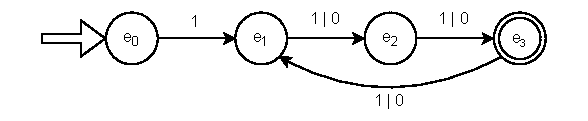
\includegraphics[width=\textwidth]{Exercices/EX2/ex2.1.drawio.pdf}
\end{minipage}

\vspace{1.5cm}
\textbf{\underline{L\(_2\)}}

\vspace{0.3cm}
\noindent
\begin{center}
\begin{minipage}{0.4\textwidth}
    \centering
    \textbf{\underline{Solution\(_1\)}}\\[0.2cm]
    S \(\to\) aAb \texttt{|} bB\\[0.1cm]
    A \(\to\) aAb \texttt{|} bB\\[0.1cm]
    \hspace{-0.6cm}    B \(\to\) bB \texttt{|} \(\epsilon\)\\[0.1cm]
\end{minipage}%
\hspace{1cm} % Adjust this value for spacing
\begin{minipage}{0.4\textwidth}
    \centering
    \textbf{\underline{Solution\(_2\)}}\\[0.2cm]
    S \(\to\) aSb \texttt{|} Sb \texttt{|} b\\[0.1cm]
\end{minipage}
\end{center}

\vspace{0.3cm}

\begin{prettyBox}{No Automaton}{red}
This grammar is neither right-regular nor left-regular, it is a Type 2 grammar.  
Therefore, it does not have a corresponding automaton.
\end{prettyBox}

\newpage
\textbf{\underline{L\(_3\)}}

    \vspace{0.3cm}

    \hspace{1.5cm}
\noindent
\begin{minipage}{0.4\textwidth}
    S \(\to\) aaS \texttt{|} cA \\[0.1cm]
    A \(\to\) bbA \texttt{|} b 
\end{minipage}%
\hspace{-1cm}
\begin{minipage}{0.5\textwidth}
    \centering
    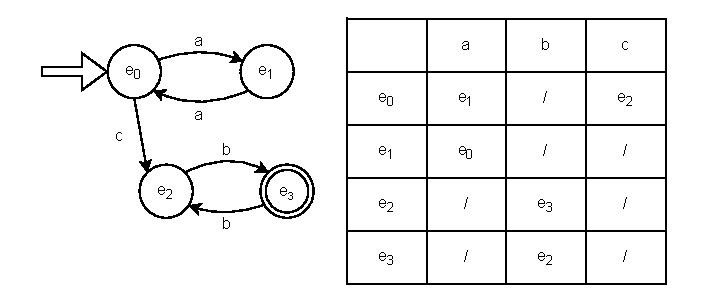
\includegraphics[width=\textwidth]{Exercices/EX2/ex2.3.drawio.pdf}
\end{minipage}

\vspace{2cm}

\textbf{\underline{Example with 'aacbb\#'}}
\begin{center} 
    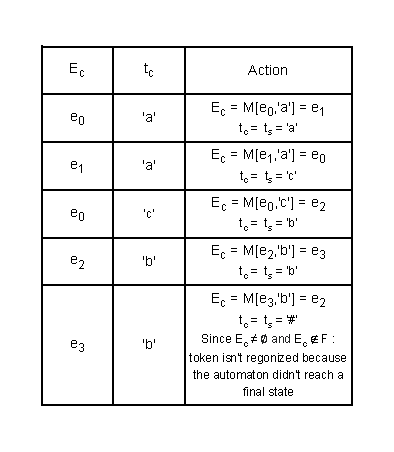
\includegraphics[height=0.5\textheight]{Exercices/EX2/ex2.3.ex.drawio.pdf}
\end{center}

